%!TEX root = ../Thesis.tex
\section{Problemanalyse (Franziska Plate)}

Durch die bereits gemeldeten Probleme der Mitarbeiter lassen sich vier
verschiedene Problemfelder abgrenzen, welche im Folgenden genauer
erläutert werden. Zum Abschluss der Problemanalyse wird ein möglicher
Soll-Zustand beschrieben und Lösungsansätze werden genannt.

Problemfeld Nummer eins ist, dass die IT-Abteilung absolut überfordert
ist. Das liegt zum einen daran, dass die IT-Ausstattung (Hard- und
Software) nicht einheitlich ist. Die Mitarbeiter müssen sich so um
verschiedene Modelle und Hersteller-Probleme kümmern und es lässt sich
beispielsweise eine Lösung für den einen Laptop nicht auf den anderen
übertragen, da dieser von einem anderen Hersteller ist. Das Gleiche
gilt für die Server in den Kellerräumen der Zentrale.

Ein weiterer Punkt, welcher zur Überforderung beiträgt ist, dass es
keine zentrale Anlaufstelle für Support-Anfragen gibt. Somit hat jeder
Mitarbeiter alle Support-Anfragen zum Bearbeiten vorliegen. Es gibt
keine Information darüber, wer welches Ticket bearbeitet, ob Tickets
priorisiert behandelt werden müssen oder wie der Stand der Tickets
momentan ist. Das führt neben der Überforderung ebenfalls zu Chaos und
Unübersichtlichkeit im Support des Unternehmens.

Eine weitere Baustelle ist der hohe Wartungsaufwand und die damit
verbundenen Wartungskosten. Ursache hierfür ist unter anderem, dass
neben den IT-Mitarbeitern auch die Mitarbeiter der Franchise-Filialen,
über eine unsichere DSL-Anbindung, auf den Sever und somit direkt auf
die Daten zugreifen können. Folgen können sein, dass wichtige Daten
versehentlich verändert werden (und es ist nicht nachvollziehbar, wer
welche Daten, wann geändert hat und vor allem warum, so ist kein
Verantwortlicher zu identifizieren. Das erhöht ebenfalls den
Wartungsaufwand der IT-Abteilung), Dritte können unerlaubt Zugriff auf
den Server bekommen oder Viren können durch die unsichere
DSL-Anbindung ins Unternehmensnetz gelangen und so Schäden
verursachen, was so für hohe Wartungskosten sorgen wird. Ein weiterer
Punkt, der im Zusammenhang mit den hohen Wartungskosten und dem hohen
Wartungsaufwand (Resultat aus der nicht-einheitlichen IT-Ausstattung)
beachtet werden muss, sind die s.g.~Total Cost of Ownership. Die Total
Cost of Ownership sind die Kosten, die über den kompletten Zeitraum
anfallen, indem man die Software oder Hardware besitzt. Also
beispielsweise die Support-, Betriebs-, Wartungs- und
Schulungskosten. So kann beispielsweise eine Software in der
Anschaffung preiswerter sein, als die anderen Software-Optionen,
allerdings können die Betriebskosten über die Lebensdauer im
Unternehmen weitaus höher sein, als die der anderen Produkte. Und so
lassen sich durch die Beachtung der Total Cost of Ownership Kosten
einsparen\footnote{Vgl.~\cite{TCO}, Online im Internet.}.

% \begin{figure}[H]
% \centering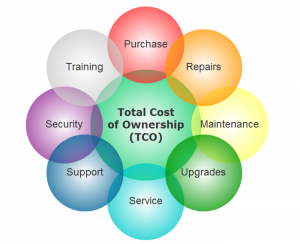
\includegraphics[width=0.3\textwidth]{img/tco}
% \caption[Bestandteile der Total Cost of Ownership]{Quelle:
%   \url{http://www.tritechamerica.com/total-cost-of-ownership/}, Stand:
%   20.04.2016}
% \end{figure}

\begin{figure}[H]
\centering
\begin{minipage}[t]{0.8\textwidth}
{\centering\fbox{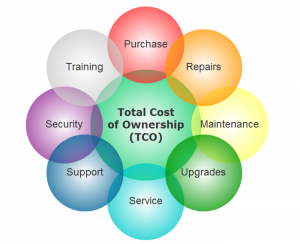
\includegraphics[width=0.7\textwidth]{img/tco}}\\}
\caption{Bestandteile der Total Cost of Ownership} % Überschrift
\source{http://www.tritechamerica.com/total-cost-of-ownership/, Stand: 20.04.2016} % Quelle
\end{minipage}
\end{figure}

Eine weitere Baustelle ist die mangelnde Datensicherheit und der
Datenschutz. Dies ist unter anderem zurückzuführen auf die unsichere
Anbindung der Franchise-Filialen, den Standort des Servers (im Keller
der Zentrale), das Accessmanagement für den Server-Zugriff (jeder
Mitarbeiter der Franchise-Filialen kann auf den Server und die
Unternehmensdaten zugreifen, da diese auf ein und demselben Server
liegen).

Ebenfalls wird deutlich, dass die Server-Architektur keinerlei
flexible Skalierbarkeit bietet, da Hardware bei Kapazitätserweiterung
erst bestellt und angeschafft werden muss. Diese neue Anschaffung und
vor allem die neue Einrichtung der Hardware kosten Zeit und
Geld. Somit ist eine flexible Skalierbarkeit unabkömmlich sobald die
Firma expandieren will beziehungsweise den Expansions-Gedanken schon
im Kopf hat.

Durch die vorhergehende Problemanalyse wird deutlich, dass vor allem
die Prozesse Optimierungspotential bieten und es muss ein interner
Standard im Bereich der Hard- und Software eingeführt werden.

Um nun die IT-Mitarbeiter zu entlasten und deren Überforderung zu
reduzieren muss zuerst eine Standardisierung der IT-Ausstattung (Hard-
und Software) vorgenommen werden. Dazu zählt, dass die verwendete
Hardware von nur einem Hersteller bezogen wird und sich die Modelle
nicht grundlegend unterscheiden. Ebenfalls muss die Software
lizenziert sein und aus einer sicheren und verlässlichen Quelle
stammen. Darüber hinaus werden so unter anderem die Wartungskosten und
der Wartungsaufwand gesenkt.

Als Lösung für die anderen Probleme, wie hoher Wartungsaufwand und
hohe Wartungskosten, mangelnder Datenschutz und Datensicherheit und
keine flexible Skalierbarkeit, bietet sich das Einführen einer Cloud
in das Unternehmensnetzwerk an. Genauer gesagt wird hier die Option
Infrastructure as a Service in Betracht gezogen und der im Keller
befindliche Server wird zu eigenen Datenbankserver auf dem die Kunden-
und Unternehmensdaten gespeichert sind.

Eine Cloud bietet mehrere Vorteile. Ein großer Vorteil ist, dass sich
eine Cloud flexibel skalieren lässt und sich so den verändernden
Unternehmensbedingungen anpassen kann. Wenn beispielsweise mehr
Speicherkapazität auf dem Cloud-Server benötigt wird, kann dies ohne
Probleme und schnell beim Cloud-Anbieter nachbestellt werden, es muss
keine zusätzliche Hardware bestellt und eingerichtet werden, da es
alles virtuell geschieht. In die andere Richtung ist die
Skalierbarkeit natürlich ebenfalls möglich. Es wird also nur das
bezahlt, was man auch wirklich braucht. Weitere Vorteile sind, dass
durch eine Cloud der Wartungs- und Upgrade-Aufwand gemindert wird, da
dies komplett der Cloud-Anbieter übernimmt. Ebenfalls wird so eine
sichere Plattform bereitgestellt und es kann über eine sichere
Verbindung mit der Cloud kommuniziert werden.

Auf dieser hybriden Cloud, das heißt, dass die Cloud sowohl aus einer
Public- (angeboten vom Cloud-Anbieter als \acrshort{IaaS}) als auch einer
Private-Cloud (eigener Server im Keller) besteht, werden nun die
benötigten Systeme (wie der Webshop oder andere IT-Systeme
(ServiceDesk, CRM, ERP und/oder Solution Manager)
bereitgestellt\footnote{Vgl.~\cite{Hybrid-Cloud}, Online im Internet.}. Die Systeme in der
Cloud erhalten ihre Daten (Kunden-, Einkaufs- oder Unternehmensdaten)
über eine sichere Verbindung mit dem Datenbankserver, welcher sich in
der Zentrale befindet. So greift keiner der Franchise-Filialen mehr
direkt auf die sensiblen Daten zu, da sie nur direkt an die Cloud
angebunden sind und lediglich Lese-Rechte auf die sensiblen Daten
haben. So werden versehentliche Änderungen in den Datensätzen
vermieden.

Neben den bereits genannten Problemlösungen müssen ebenfalls die
Prozesse an den neuen Standard angepasst, optimiert und überarbeitet
werden, um so letztendlich auch beispielsweise vereinbarte \acrshort{SLA}’s
einhalten zu können. Hierfür muss das Rad nicht neu erfunden werden,
sondern es kann sich an ITIL bedient werden. ITIL ist eine Sammlung
von vordefinierten und standardisierten Prozessen, Funktionen und
Rollen. Es bietet Best-Practice Vorschläge, welche an das Unternehmen
angepasst werden können bzw.~müssen und eignet sich somit perfekt für
ein Start-up. ITIL besteht aus fünf ,,Phasen'', welche den
Service-Lifecycle widerspiegeln: Service Strategy (Servicestrategie),
Service Design (Serviceentwurf), Service Transition
(Serviceüberführung), Service Operation (Servicebetrieb) und Continual
Service Improvement (kontinuierliche
Serviceverbesserung)\footnote{Vgl.~\cite{ITIL-Prozesse}, Online im Internet}. Beispiele
für ITIL-Standards bzw. Best-Practice Prozesse wären: das Business
Relationship Management (Service
Strategy\footnote{Vgl.~\cite{ITIL-Service-Strategy}, Online im Internet}) das Service
Level-, Risiko-, Compliance-, Supplier – Management (Service
Design\footnote{Vgl.~\cite{ITIL-Service-Design}, Online im Internet}) das Change-,
Release-, Configuration – Management (Service
Transition\footnote{Vgl.~\cite{ITIL-Service-Transition}, Online im Internet}), der
ServiceDesk bzw. Incident-, Problem-, Access-, Event – Management
(Service Operation\footnote{Vgl.~\cite{ITIL-Service-Operation}, Online im Internet}) und
Service Reviews (Continual Service
Improvement\footnote{Vgl.~\cite{ITIL-CSI}, Online im Internet}).

Die vordefinierten Standards in ITIL können flexibel an das
Unternehmen ,,Stylez'' angepasst werden und helfen somit die Prozesse
zu optimieren und zu strukturieren und ,,Stylez'' kann sich an
vordefinierte Standards und Best-Practices bedienen und diese nutzen.

Abschließend lässt sich sagen, dass mit den erwähnten
Änderungsmaßnahmen alle Problemfelder, welche analysiert wurden
abgedeckt und behoben werden können.

Um nun die Veränderungen durchzuführen, kann sich ,,Stylez'' an den
vordefinierten Standards in ITIL für das Change Management bedienen
und kann diese an seine Bedürfnisse anpassen.
